\section{Circular Polization} \label{sec:clas.polar}

As mentioned in Sec.~\ref{sec:clas.acc}, the electron beam provided by \abbr{CEBAF} has the capability of having 75\% longitudinal polarization. Longitudinal polarized electrons produce circularly polarized photons when the electrons are incident on a high-Z material. The experiment \g12 used a Au foil as a radiator therefore \g12 had a circular polarized beam. The circular polarization production process is quantum mechanical. From QED calculations, the degree of circular polarization transfer to the photon, $P_{circ}$, is seen to depend on the ratio of the relative electron energy to the bremsstrahlung photon, $\epsilon$:
\begin{equation}\label{eq:polarization}
	P_{circ} = (\frac{4\epsilon - \epsilon^{2}}{4-4\epsilon+3\epsilon^{2}})P_{e} 
\end{equation}
where $\epsilon = k/E_{0}$, $k$ is the bremsstrahlung photon energy and $E_{0}$ is the incident electron energy. Equation~\ref{eq:polarization} shows that circular polarization of the photon is transferred directly from the polarization of the electron, it also shows that the atomic nucleus or radiator plays no role in transfer of polarization. The transfer of circular polarization is maximum at the higher end of the energy spectrum $\epsilon$ and decreases towards the lower end of the spectrum as seen in Fig.~\ref{fig:jlab.polarization}. Figure~\ref{fig:jlab.polarization} also illustrates that polarization transfer is favored when the radiated photons take up large fractions of the incident electron energy. Coulomb and screening corrections (due to the atomic electrons) do not significantly affect the polarization of the emitted photons. 

\begin{figure}[h!]\begin{center}
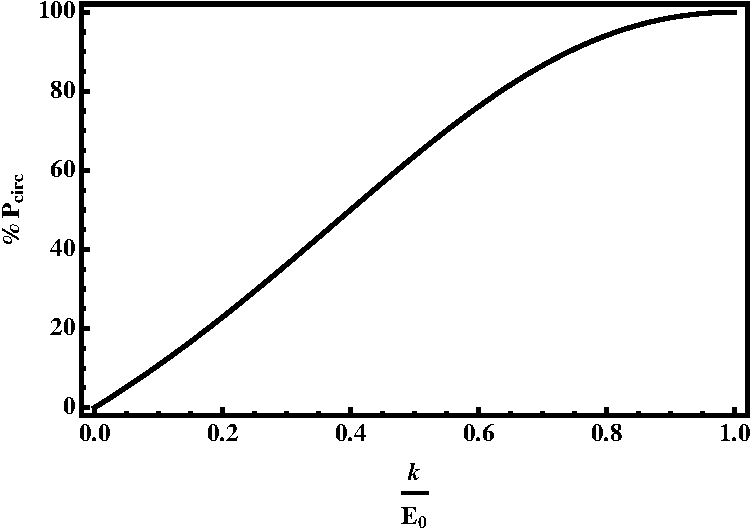
\includegraphics[width=0.8\figwidth,height=\qfigheight]{\grpath/hall-b/polarization.pdf}
\caption[Circular polarization Graph]{\label{fig:jlab.polarization}QED calculation for the degree of circular polarization of 50-MeV electrons in lead. The curve shown is a Born-approximated calculation which neglects screening corrections. An exact calculation involving Coulomb and screening corrections (not shown) yields similar results.\cite{Olsen}}
\end{center}\end{figure}
